
\documentclass[a4paper,12pt]{article} 
\usepackage[top = 2.5cm, bottom = 2.5cm, left = 2.5cm, right = 2.5cm]{geometry} 
\usepackage[T1]{fontenc}
\usepackage[utf8]{inputenc}
\usepackage{multirow} 
\usepackage{amsmath}
\usepackage{amssymb}
\usepackage{booktabs} 
\usepackage{graphicx}  
\usepackage{subfig}
\usepackage{setspace}
\setlength{\parindent}{0in}
\usepackage{float}
\usepackage{tablefootnote}
\usepackage{fancyhdr}
\usepackage[english]{babel}
\usepackage{xcolor}
\usepackage{multirow}
\usepackage{listings}
\usepackage{dcolumn}
\lstset{
  basicstyle=\footnotesize\ttfamily,
  columns=fullflexible,
  frame=single,
  breaklines=true,
  postbreak=\mbox{\textcolor{red}{$\hookrightarrow$}\space},
}
\usepackage{hyperref}
 \hypersetup{
     colorlinks=true,
     linkcolor=black,
     filecolor=black,
     citecolor = black,      
     urlcolor=blue,
     }
\usepackage{csvsimple}
\pagestyle{fancy} 
\fancyhf{} 
\lhead{\footnotesize Economics 714: Replication}
\rhead{\footnotesize Javier Tasso} 
\cfoot{\footnotesize \thepage} 




\begin{document}





\begin{tabular}{p{15.5cm}} 
{\large \bf Economics 714 - Computational Methods in Economics} \\
University of Pennsylvania \\ Fall 2021 \\ \\ 
\hline 
\\
\end{tabular} 

\vspace*{0.3cm} 

\begin{center} 
	{\Large \bf Replication} 
	\vspace{2mm}
	
        
	{\bf Javier Tasso} 
		
\end{center}  

\vspace{0.4cm}

%%%%%%%%%%%%%%%%%%%%%%%%%%%%%%%%%%%%%%%%%%%%%%%%
%%%%%%%%%%%%%%%%%%%%%%%%%%%%%%%%%%%%%%%%%%%%%%%%


\section*{Introduction}

Originally we planned to replicate Eaton \& Kortum (2002) using data from Kortum's website \href{http://kortum.elisites.yale.edu/home/technology-geography-and-trade
}{here}. We couldn't open most of the trade data needed to do the replication, so we choose to (try to) replicate Waugh (2010) instead. In the first section we verify that the gravity data Waugh has in his repository matches the relationship found in Eaton \& Kortum and also that it is consistent with our intuition. In section $2$ we combine datasets, plot some information and estimate the preliminary value of $\theta$ which is our parameter of interest. Section $3$ tries to replicate the results of the geographical barriers of Waugh. We couldn't replicate them, but we added a slight modification and tried to say something about the size of the economy and trade shares using his methods. Finally section $4$ tries to diagnose what went wrong by looking at the data and the constructed measures we used in previous sections. Even though we weren't successful in the replication, we wanted to present the results anyways to show our work. 


\begin{itemize}
    \item Gravity data and country names were obtained from \href{https://github.com/mwaugh0328/Gravity-Estimation}{this repository} that belongs to Mike Waugh. 
    
    \item Price data as well as other inputs were downloaded from \href{https://www.openicpsr.org/openicpsr/project/112382/version/V1/view?path=/openicpsr/112382/fcr:versions/V1/data_code_AER_20070560/Data&type=folder}{here}.
    
    \item Click \href{https://github.com/javiertasso/econ714_replication_tasso}{here} for the repository. Every input needed should be there and the codes themselves generate all the output for the tex file. 
    
    
    
\end{itemize}

\section{Preliminary Data}

 For this section we took advantage of the file \textit{gravity\_data.txt} located at \href{https://github.com/mwaugh0328/Gravity-Estimation}{this repository}. Code \textit{1\_replication\_Eaton\_Kortum.R} loads the data and generates figure (\ref{EKfig1_distance_norm_import_share}). This figure should be similar to figure (1) in Eaton \& Kortum ($2002$). We see a negative relationship between the normalized import share and distance. There are three countries missing (relative to Eaton Kortum ($2002$)) so the figure is not exactly the same. This relationship we see in figure (\ref{EKfig1_distance_norm_import_share}) makes sense: as distance increases, the normalized import shares falls because things become more expensive. 
  
 % First I replicate figure (1) of Eaton-Kortum. Figure  does the job. 
 
  \begin{figure}[htbp!]
     \centering
     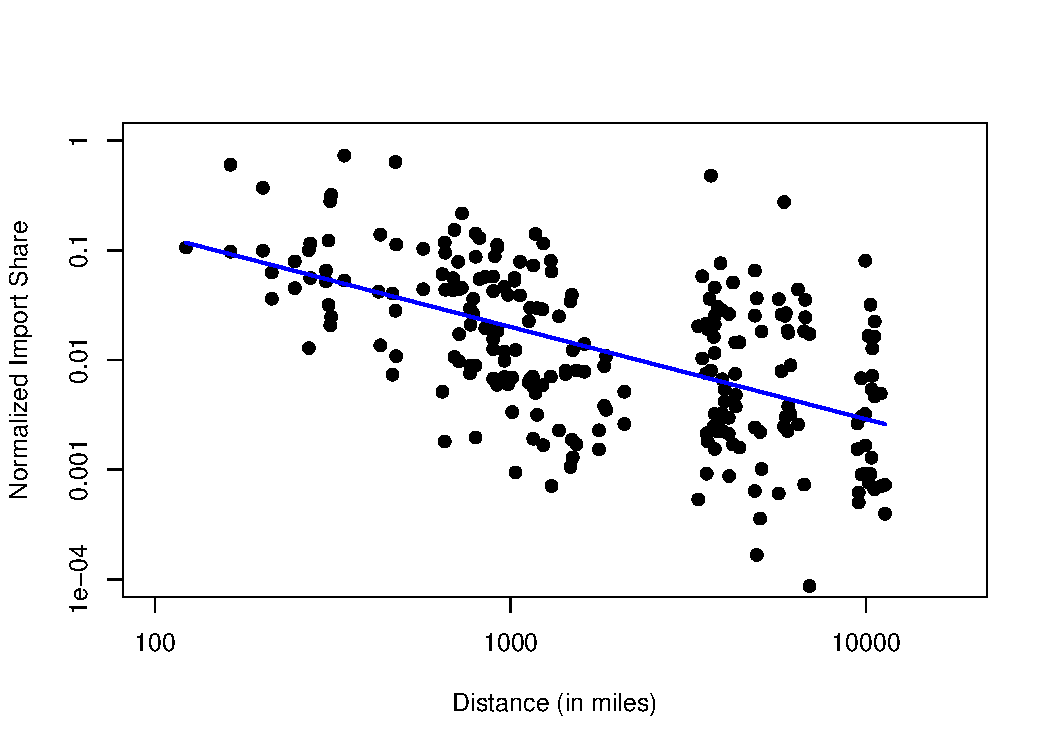
\includegraphics[scale=0.75]{distance_and_normalized_import_share_EK_fig_1.pdf}
     \caption{Distance and Normalized Import Shares}
     \label{EKfig1_distance_norm_import_share}
 \end{figure}
 
 \section{Construction of the Price Measure}
 
 To construct the price measure we follow Waugh (2010). All the data can be downloaded from \href{https://www.openicpsr.org/openicpsr/project/112382/version/V1/view?path=/openicpsr/112382/fcr:versions/V1/data_code_AER_20070560/Data&type=folder}{this link}. Code \textit{2\_replication\_Waugh.R} generates all the output of this section. Table (\ref{table_1_waugh}) corresponds to table ($1$) in the paper and presents the trade shares in $1996$ for selected countries. 
 
 % latex table generated in R 3.6.1 by xtable 1.8-4 package
% Tue Dec 14 15:32:03 2021
\begin{table}[!htbp]
\centering
\begin{tabular}{ccccccccc}
  \hline
 & USA & CAN & CHN & JPN & MEX & MWI & SEN & ZAR \\ 
  \hline
USA & 83.25 & 39.74 & 3.63 & 2.27 & 31.63 & 1.58 & 2.16 & 2.93 \\ 
  CAN & 3.79 & 49.21 & 0.32 & 0.22 & 0.72 & 0.67 & 0.57 & 0.51 \\ 
  CHN & 1.79 & 1.42 & 77.61 & 1.45 & 0.31 & 2.51 & 2.70 & 6.81 \\ 
  JPN & 3.04 & 2.01 & 7.00 & 92.56 & 1.60 & 2.65 & 1.34 & 0.82 \\ 
  MEX & 1.89 & 1.34 & 0.06 & 0.02 & 61.10 & 0.00 & 0.01 & 0.01 \\ 
  MWI & 0.00 & 0.00 & 0.00 & 0.00 & 0.00 & 41.52 & 0.00 & 0.00 \\ 
  SEN & 0.00 & 0.00 & 0.00 & 0.00 & 0.00 & 0.00 & 52.68 & 0.00 \\ 
  ZAR & 0.00 & 0.01 & 0.00 & 0.00 & 0.00 & 0.00 & 0.00 & 51.53 \\ 
   \hline
\end{tabular}
\caption{1996 Trade Shares for Selected Countries} 
\label{table_1_waugh}
\end{table}

 
 Figures (\ref{raw_scatterplot_figure_1_prices_and_GDP}) and (\ref{scatterplot_figure_1_prices_and_GDP}) are equivalent to figure ($1$) in the paper. Note that figure (\ref{scatterplot_figure_1_prices_and_GDP}) has a different scale on the axis. 
 
 \begin{figure}[htbp!]
     \centering
     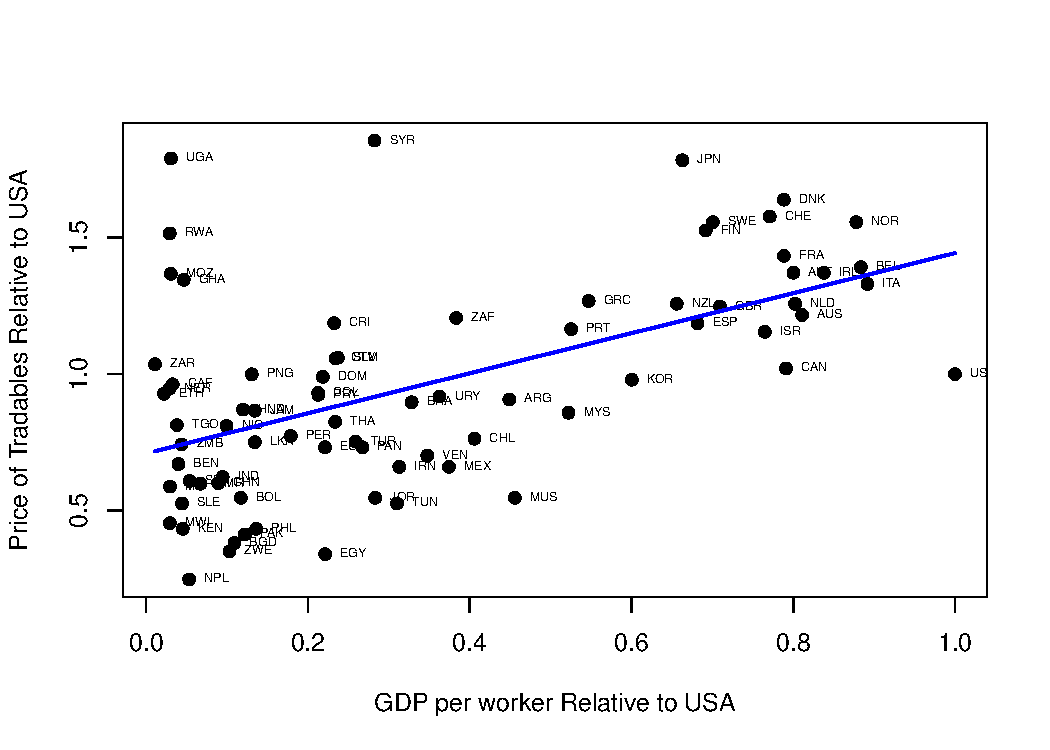
\includegraphics[scale=0.75]{raw_scatterplot_figure_1.pdf}
     \caption{Price of Tradables and GDP}
     \label{raw_scatterplot_figure_1_prices_and_GDP}
 \end{figure}
 
  \begin{figure}[htbp!]
     \centering
     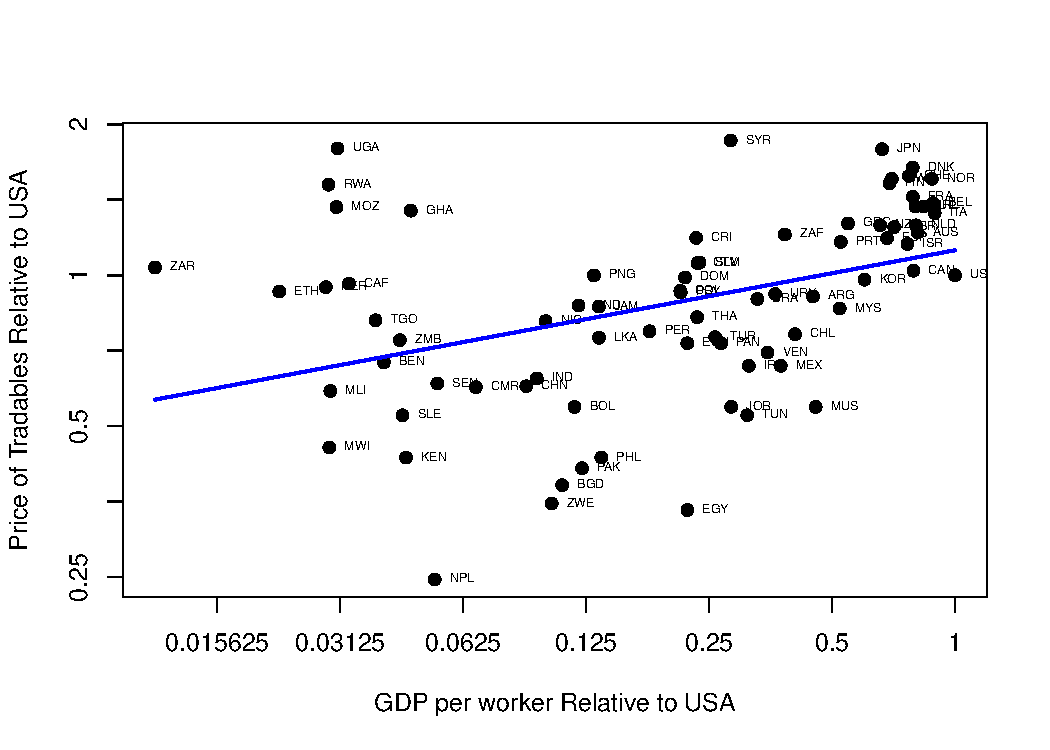
\includegraphics[scale=0.75]{scatterplot_figure_1.pdf}
     \caption{Price of Tradables and GDP - Log Scale}
     \label{scatterplot_figure_1_prices_and_GDP}
 \end{figure}
 
 Let $X_{ij}$ be the the amount of goods (aggregated somehow) that country $j$ imports from country $i$ and let $X_{jj}$ be the amount of goods that country $j$ buys from itself. Next define $p_j$ and $p_i$ price indexes and $\tau_{ij}$ a parameter that governs trade costs. Then we have the following relationship which is equation (4) in the paper. . 
 
 \begin{align*}
     \frac{X_{ij}}{X_{jj}} & = \bigg(\tau_{ij}\cdot \frac{p_j}{p_i}\bigg)^{-\frac{1}{\theta}}
 \end{align*}
 
 Note that the right hand side is a factor that takes into account the relative prices between home and country $i$, the trade costs possible arising from distance and other barriers and a parameter $\theta>0$. $\theta$ is a parameter that controls the strength of the comparative advantage of the countries and we want to estimate it. Take logs to get the following. 
 
 \begin{align}\label{baseline_regression_with_no_intercept}
     \ln\bigg(\frac{X_{ij}}{X_{jj}}\bigg) & = -\frac{1}{\theta} \cdot \ln (\hat{\tau}_{ij}) 
 \end{align}
 
 The left hand side is observed. We will recover from data $\ln(\hat{\tau}_{ij})$ and then run a regression with no intercept to get an estimate for $\theta$. The next step is to construct this measure that involves prices. Let $l$ be an index for goods from price information we will construct that measure as follows. $\max^2$ represents the second highest value. 
 
 \begin{align*}
     \ln(\hat{\tau}_{ij}) & = \max_{l}^2 \quad \{\ln(p_i(l)) - \ln(p_j(l))\}
 \end{align*}
 
 For each pair of countries $(i,j)$ we are choosing the good that makes the relative price the highest, using the second maximum to get a better measure. That's going to give us an idea of the trade costs between countries $(i,j)$. We expect a negative relationship between normalized trade shares (measured in logs) and the measure of $\tau$ constructed from price data (also measured in logs). We see that in figure (\ref{trade_shares_and_tau}). 
 
   \begin{figure}[htbp!]
     \centering
     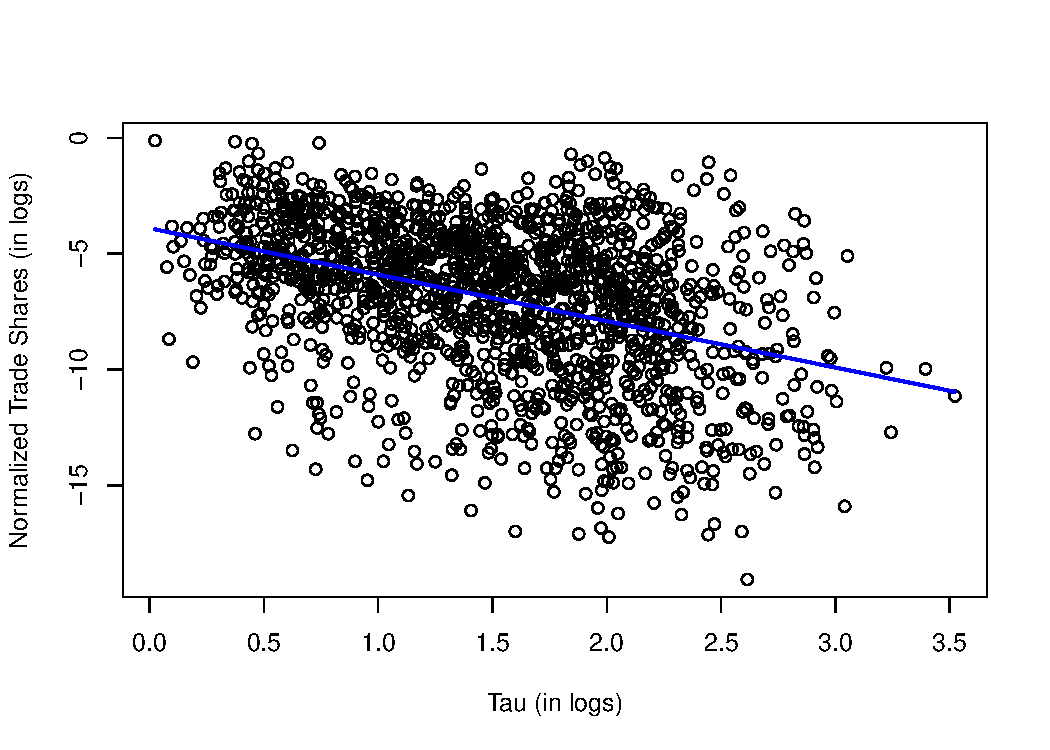
\includegraphics[scale=0.75]{trade_shares_and_tau.pdf}
     \caption{Trade Shares and $\tau$}
     \label{trade_shares_and_tau}
 \end{figure}
 
 Figure (\ref{trade_shares_and_tau}) was generated in \textit{2\_replication\_Waugh.R}. The code reshapes and merges different datasets that will be used in next section. Next we regress the normalized trade shares in our measure of $\hat{\tau}$ without intercept to get the results of table (\ref{linear_model_for_theta}). These results imply a $\hat{\theta} \simeq 0.24$ which differs from the one found in Waugh ($2010$). We will continue with the analysis and then see if we can find the reason why we get different results. 
 
 
% Table created by stargazer v.5.2.2 by Marek Hlavac, Harvard University. E-mail: hlavac at fas.harvard.edu
% Date and time: Tue, Dec 14, 2021 - 3:32:05 PM
% Requires LaTeX packages: dcolumn 
\begin{table}[!htbp] \centering 
  \caption{First Estimate of Theta} 
  \label{} 
\begin{tabular}{@{\extracolsep{5pt}}lD{.}{.}{-3} } 
\\[-1.8ex]\hline 
\hline \\[-1.8ex] 
 & \multicolumn{1}{c}{\textit{Dependent variable:}} \\ 
\cline{2-2} 
\\[-1.8ex] & \multicolumn{1}{c}{Trade Share (in logs)} \\ 
\hline \\[-1.8ex] 
 Tau (in logs) & -4.189^{***} \\ 
  & (0.054) \\ 
  & \\ 
\hline \\[-1.8ex] 
Observations & \multicolumn{1}{c}{1,592} \\ 
R$^{2}$ & \multicolumn{1}{c}{0.805} \\ 
Adjusted R$^{2}$ & \multicolumn{1}{c}{0.804} \\ 
\hline 
\hline \\[-1.8ex] 
\textit{Note:}  & \multicolumn{1}{r}{$^{*}$p$<$0.1; $^{**}$p$<$0.05; $^{***}$p$<$0.01} \\ 
\end{tabular} 
\end{table} 
\label{linear_model_for_theta}
 
 \section{Different Regressions} 
    
 Code \textit{3\_replication\_Waugh.R} does everything for this section. In the first part of the code we generate dummy variables for different levels of distance (in miles) this will help us divide the sample in $6$ groups depending on how close or how far apart are two countries. The groups are $\text{dist}<375$, $375\leq \text{dist} < 750$, $750\leq \text{dist} < 1500$, $1500\leq \text{dist} < 3000$, $3000\leq \text{dist} < 6000$ and $6000\leq \text{dist}$. We weren't able to replicate the results from table $(2)$ of Waugh's paper, but we will present some estimations in this section and then try to discover what went wrong. We want to extend equation (\ref{baseline_regression_with_no_intercept}) allowing for different intercepts (fixed effects for importers and exporters), and controlling for distance to see the behaviour of the coefficient next to the constructed $\ln(\hat{\tau}_{ij})$. Table (\ref{models_theta}) shows the results. 
 
 
% Table created by stargazer v.5.2.2 by Marek Hlavac, Harvard University. E-mail: hlavac at fas.harvard.edu
% Date and time: Tue, Dec 14, 2021 - 6:19:17 PM
% Requires LaTeX packages: dcolumn 
\begin{table}[!htbp] \centering 
  \caption{Estimates of Theta - Different Models} 
  \label{models_theta} 
\begin{tabular}{@{\extracolsep{5pt}}lD{.}{.}{-3} D{.}{.}{-3} D{.}{.}{-3} D{.}{.}{-3} } 
\\[-1.8ex]\hline 
\hline \\[-1.8ex] 
 & \multicolumn{4}{c}{\textit{Dependent variable:}} \\ 
\cline{2-5} 
\\[-1.8ex] & \multicolumn{4}{c}{Trade Share (in logs)} \\ 
 & \multicolumn{1}{c}{No FE} & \multicolumn{1}{c}{FE exporter} & \multicolumn{1}{c}{FE importer} & \multicolumn{1}{c}{FE both} \\ 
\\[-1.8ex] & \multicolumn{1}{c}{(1)} & \multicolumn{1}{c}{(2)} & \multicolumn{1}{c}{(3)} & \multicolumn{1}{c}{(4)}\\ 
\hline \\[-1.8ex] 
 Tau (in logs) & -1.703^{***} & -0.402^{***} & -2.015^{***} & -0.301^{***} \\ 
  & (0.123) & (0.079) & (0.128) & (0.083) \\ 
  & & & & \\ 
 Dist 1 & -1.019 & -7.503^{***} & 1.328 & -3.601^{***} \\ 
  & (0.964) & (0.594) & (1.039) & (0.576) \\ 
  & & & & \\ 
 Dist 2 & -2.364^{***} & -7.001^{***} & 0.288 & -1.972^{***} \\ 
  & (0.651) & (0.433) & (0.779) & (0.448) \\ 
  & & & & \\ 
 Dist 3 & -2.812^{***} & -7.777^{***} & -0.143 & -2.844^{***} \\ 
  & (0.313) & (0.323) & (0.592) & (0.371) \\ 
  & & & & \\ 
 Dist 4 & -3.613^{***} & -8.178^{***} & -0.975^{*} & -3.109^{***} \\ 
  & (0.270) & (0.308) & (0.567) & (0.357) \\ 
  & & & & \\ 
 Dist 5 & -4.502^{***} & -8.716^{***} & -2.431^{***} & -4.043^{***} \\ 
  & (0.255) & (0.308) & (0.566) & (0.355) \\ 
  & & & & \\ 
 Dist 6 & -4.778^{***} & -9.618^{***} & -2.212^{***} & -4.802^{***} \\ 
  & (0.220) & (0.296) & (0.545) & (0.339) \\ 
  & & & & \\ 
 Shared Border & 0.102 & 0.380 & 0.118 & 0.639^{**} \\ 
  & (0.587) & (0.317) & (0.540) & (0.272) \\ 
  & & & & \\ 
\hline \\[-1.8ex] 
Observations & \multicolumn{1}{c}{1,557} & \multicolumn{1}{c}{1,557} & \multicolumn{1}{c}{1,557} & \multicolumn{1}{c}{1,557} \\ 
R$^{2}$ & \multicolumn{1}{c}{0.853} & \multicolumn{1}{c}{0.960} & \multicolumn{1}{c}{0.883} & \multicolumn{1}{c}{0.972} \\ 
Adjusted R$^{2}$ & \multicolumn{1}{c}{0.852} & \multicolumn{1}{c}{0.958} & \multicolumn{1}{c}{0.879} & \multicolumn{1}{c}{0.970} \\ 
\hline 
\hline \\[-1.8ex] 
\textit{Note:}  & \multicolumn{4}{r}{$^{*}$p$<$0.1; $^{**}$p$<$0.05; $^{***}$p$<$0.01} \\ 
\end{tabular} 
\end{table} 

 
 From table (\ref{models_theta}) we learn that controlling for distance and allowing for different intercepts changes the estimates of $\theta$ by a lot. The theory predicts that we should not have an intercept, but it does not seem to fit the data so well. We could already see that in figure (\ref{trade_shares_and_tau}) where the intercept of the line does not seem to be zero at all. Following Waugh we want to check the correlation between exporter fixed effects (or importer fixed effects) and GDP per worker. Figure (\ref{exporterFEandGDP}) plots the exporter fixed effects against GDP. This figure should be similar to figure ($2$) in Waugh ($2010$).  % There is a positive correlation meaning that countries with higher GDP yield to a higher estimate of the constant of model ($2$). Since the dependent variable is normalized trade share, we could rationalize this result by saying that higher countries trade relatively more. In our context this means that 
 
\begin{figure}[htbp!]
     \centering
     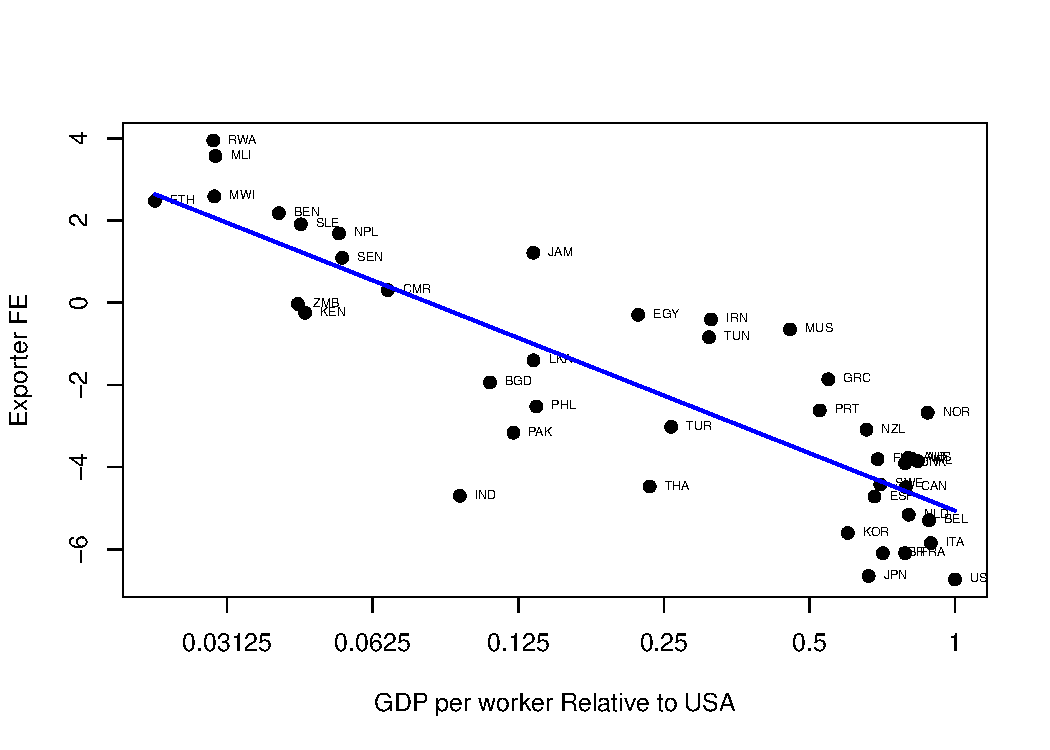
\includegraphics[scale=0.75]{exporter_FE_and_GDP.pdf}
     \caption{Exporter FE and GDP}
     \label{exporterFEandGDP}
 \end{figure}
 
 To get a better understanding of what is going on here, we are estimating a relationship that has the following form. 
 
 \begin{align}
     \ln\bigg(\frac{X_{ij}}{X_{ii}}\bigg) & = - S_i - \frac{1}{\theta} \ln(\hat{\tau}_{ij})
 \end{align}
 
 From our estimates we recover $-S_i$ for each country and then we are correlating that with GDP. Trade cost have the same impact on normalized trade shares (this is given by $-1/\theta$), but the relationship has different constants and these constants are correlated with GDP. A similar relationship is true for importer fixed effects as we can see in figure (\ref{importerFEandGDP}). % If a country has a higher GDP, then the constant is smaller  
 
 
 
 
 \begin{figure}[htbp!]
     \centering
     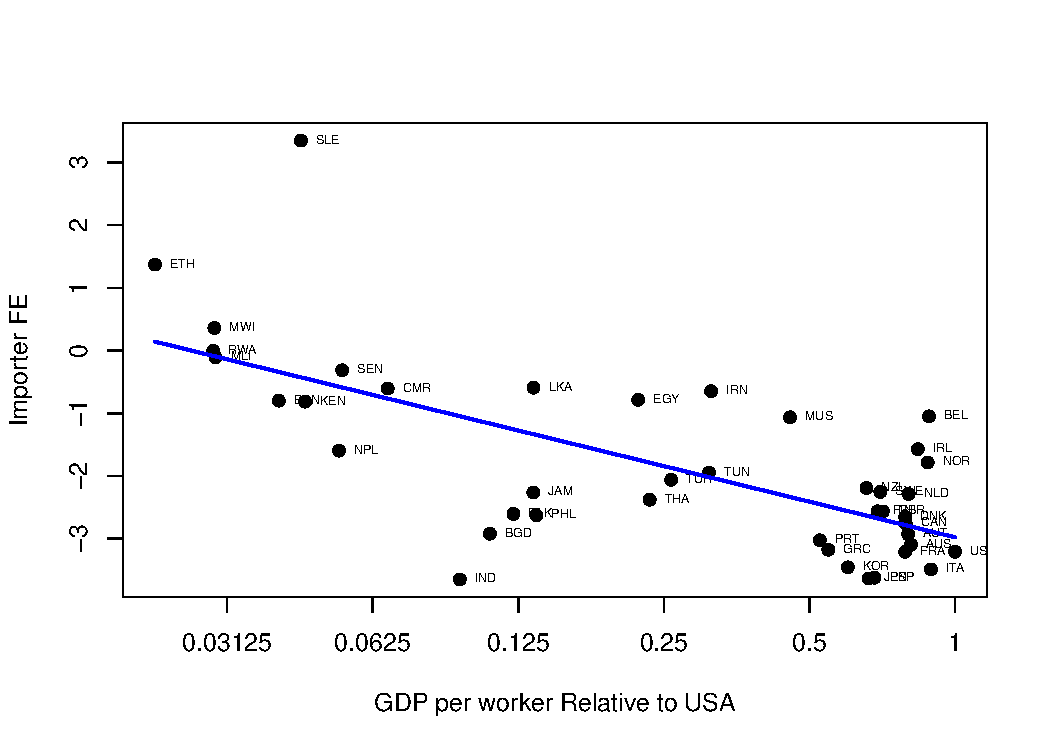
\includegraphics[scale=0.75]{importer_FE_and_GDP.pdf}
     \caption{Importer FE and GDP}
     \label{importerFEandGDP}
 \end{figure}
 
 Here we are estimating a model that looks like the following equation, but including dummies for distance and border. GDP correlates positively with these measures too. 
 
 \begin{align}
     \ln\bigg(\frac{X_{ij}}{X_{ii}}\bigg) & =  S_j - \frac{1}{\theta} \ln(\hat{\tau}_{ij})
 \end{align}
 
 We believe that Waugh (2010) does not include $\tau$ in the regression when trying to explain the geographical barriers of table $2$. Table (\ref{models_geo}) here is the equivalent of that analysis. We see that a higher distance is associated with a smaller normalized trade share, but we weren't able to replicate the same results. Next section will try to identify mistakes in our analysis. 
 
 
% Table created by stargazer v.5.2.2 by Marek Hlavac, Harvard University. E-mail: hlavac at fas.harvard.edu
% Date and time: Tue, Dec 14, 2021 - 6:21:07 PM
% Requires LaTeX packages: dcolumn 
\begin{table}[!htbp] \centering 
  \caption{Geographic Barriers} 
  \label{models_geo} 
\begin{tabular}{@{\extracolsep{5pt}}lD{.}{.}{-3} D{.}{.}{-3} D{.}{.}{-3} D{.}{.}{-3} } 
\\[-1.8ex]\hline 
\hline \\[-1.8ex] 
 & \multicolumn{4}{c}{\textit{Dependent variable:}} \\ 
\cline{2-5} 
\\[-1.8ex] & \multicolumn{4}{c}{Trade Share (in logs)} \\ 
 & \multicolumn{1}{c}{No FE} & \multicolumn{1}{c}{FE exporter} & \multicolumn{1}{c}{FE importer} & \multicolumn{1}{c}{FE both} \\ 
\\[-1.8ex] & \multicolumn{1}{c}{(1)} & \multicolumn{1}{c}{(2)} & \multicolumn{1}{c}{(3)} & \multicolumn{1}{c}{(4)}\\ 
\hline \\[-1.8ex] 
 Dist 1 & -1.901^{*} & -7.827^{***} & 0.255 & -9.087^{***} \\ 
  & (1.018) & (0.595) & (1.118) & (0.565) \\ 
  & & & & \\ 
 Dist 2 & -3.701^{***} & -7.453^{***} & -1.088 & -7.506^{***} \\ 
  & (0.682) & (0.427) & (0.835) & (0.429) \\ 
  & & & & \\ 
 Dist 3 & -4.390^{***} & -8.264^{***} & -1.786^{***} & -8.398^{***} \\ 
  & (0.308) & (0.311) & (0.629) & (0.352) \\ 
  & & & & \\ 
 Dist 4 & -5.691^{***} & -8.760^{***} & -3.209^{***} & -8.727^{***} \\ 
  & (0.238) & (0.289) & (0.592) & (0.334) \\ 
  & & & & \\ 
 Dist 5 & -7.359^{***} & -9.449^{***} & -5.617^{***} & -9.762^{***} \\ 
  & (0.158) & (0.275) & (0.570) & (0.327) \\ 
  & & & & \\ 
 Dist 6 & -7.475^{***} & -10.348^{***} & -5.398^{***} & -10.566^{***} \\ 
  & (0.108) & (0.261) & (0.546) & (0.306) \\ 
  & & & & \\ 
 Shared Border & 0.001 & 0.370 & -0.011 & 0.639^{**} \\ 
  & (0.621) & (0.320) & (0.583) & (0.274) \\ 
  & & & & \\ 
\hline \\[-1.8ex] 
Observations & \multicolumn{1}{c}{1,557} & \multicolumn{1}{c}{1,557} & \multicolumn{1}{c}{1,557} & \multicolumn{1}{c}{1,557} \\ 
R$^{2}$ & \multicolumn{1}{c}{0.835} & \multicolumn{1}{c}{0.959} & \multicolumn{1}{c}{0.863} & \multicolumn{1}{c}{0.972} \\ 
Adjusted R$^{2}$ & \multicolumn{1}{c}{0.834} & \multicolumn{1}{c}{0.958} & \multicolumn{1}{c}{0.859} & \multicolumn{1}{c}{0.970} \\ 
\hline 
\hline \\[-1.8ex] 
\textit{Note:}  & \multicolumn{4}{r}{$^{*}$p$<$0.1; $^{**}$p$<$0.05; $^{***}$p$<$0.01} \\ 
\end{tabular} 
\end{table} 

 
 \section{Diagnosis}
 
 Something went wrong during the replication. In this section we want to see if we can spot the mistake. We consider three possible problems. 
 
 \begin{enumerate}
     \item The measure $\ln(\hat{\tau}_{ij})$ doesn't behave well with respect to distance. 
     \item The measure $\ln(\hat{\tau}_{ij})$ doesn't behave well with respect to trade shares. We consider all the sample or only OECD countries to check for this issue. 
     \item Sample is different. To address this we repeat the analysis using only OECD countries. 
 \end{enumerate}
 
 % We think that something may be wrong with the way we constructed $\ln(\hat{\tau}_{ij})$. The goal of this section is to check if the measure $\ln(\hat{\tau}_{ij})$ makes sense. 
 
 First let's find the correlation between this variable and distance (also measured in logs). We should find a positive relationship, as distance increases costs are higher. That's what we see in figure (\ref{distance_and_tau}). 
 
  \begin{figure}[htbp!]
     \centering
     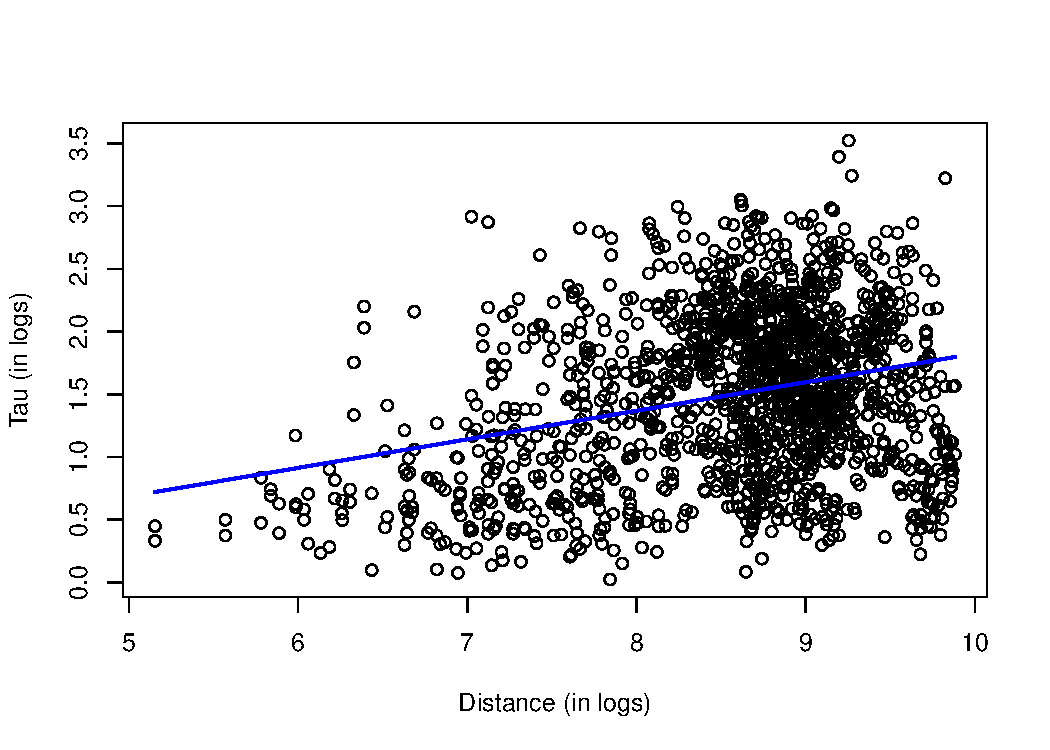
\includegraphics[scale=0.75]{distance_and_tau_hat.pdf}
     \caption{Correlation between Distance and $\tau$}
     \label{distance_and_tau}
 \end{figure}
 
 As $\tau_{ij}$ increases the normalized trade share should decrease. Here we should get something similar to figure ($2$) of Eaton Kortum ($2002$). We think we get something similar as we saw in figure (\ref{trade_shares_and_tau}) before. If we restrict the attention to OECD countries we get something that has the flavour of EK ($2002$) plot but with a different measure for the $D_{ni}$. See figure (\ref{trade_shares_and_tau_only_OECD}). 

    
  \begin{figure}[htbp!]
     \centering
     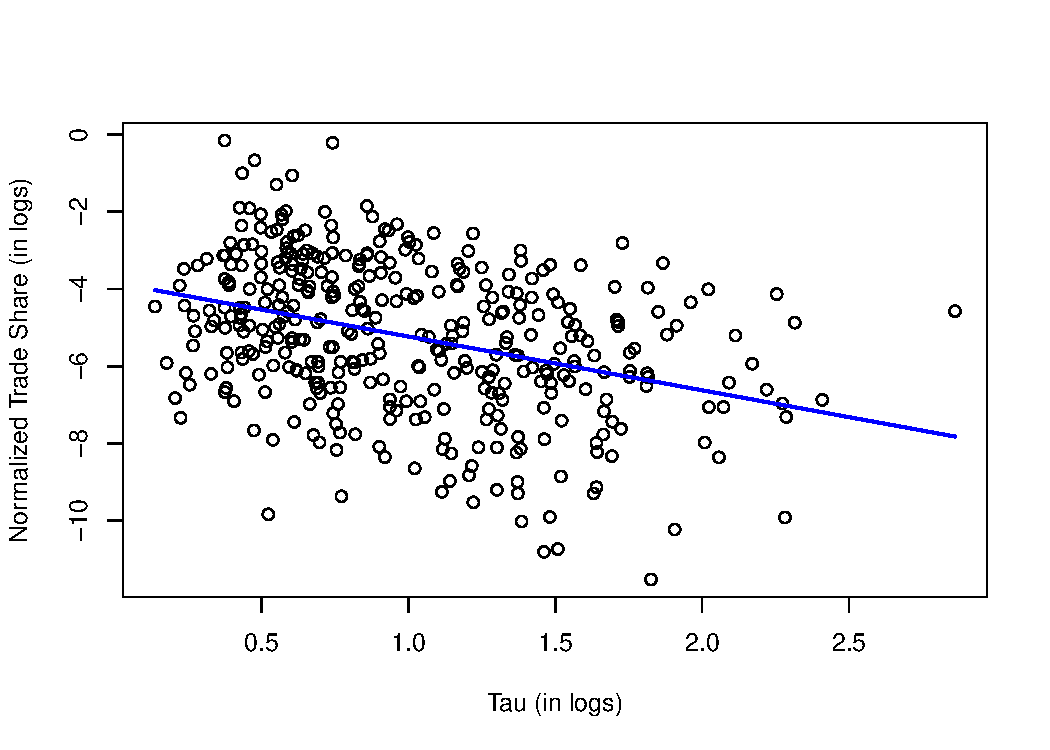
\includegraphics[scale=0.75]{tau_and_norm_trade_share_OECD.pdf}
     \caption{Correlation between Trade Shares and $\tau$} 
     \label{trade_shares_and_tau_only_OECD}
 \end{figure}
 
 Finally we want to check if using only OECD data improve the results and make them closer to the ones in the paper. Table (\ref{models_geo_OECD}) presents the geographical barriers regressions. The estimates have the same sign but the magnitudes are different. 
 
 
% Table created by stargazer v.5.2.2 by Marek Hlavac, Harvard University. E-mail: hlavac at fas.harvard.edu
% Date and time: Tue, Dec 14, 2021 - 6:36:41 PM
% Requires LaTeX packages: dcolumn 
\begin{table}[!htbp] \centering 
  \caption{Geographic Barriers} 
  \label{models_geo_OECD} 
\begin{tabular}{@{\extracolsep{5pt}}lD{.}{.}{-3} D{.}{.}{-3} D{.}{.}{-3} D{.}{.}{-3} } 
\\[-1.8ex]\hline 
\hline \\[-1.8ex] 
 & \multicolumn{4}{c}{\textit{Dependent variable:}} \\ 
\cline{2-5} 
\\[-1.8ex] & \multicolumn{4}{c}{Trade Share (in logs)} \\ 
 & \multicolumn{1}{c}{No FE} & \multicolumn{1}{c}{FE exporter} & \multicolumn{1}{c}{FE importer} & \multicolumn{1}{c}{FE both} \\ 
\\[-1.8ex] & \multicolumn{1}{c}{(1)} & \multicolumn{1}{c}{(2)} & \multicolumn{1}{c}{(3)} & \multicolumn{1}{c}{(4)}\\ 
\hline \\[-1.8ex] 
 Dist 1 & -2.211^{***} & -0.584 & -3.079^{***} & -0.252 \\ 
  & (0.717) & (0.472) & (0.833) & (0.443) \\ 
  & & & & \\ 
 Dist 2 & -3.228^{***} & -0.297 & -4.096^{***} & 0.281 \\ 
  & (0.577) & (0.392) & (0.695) & (0.374) \\ 
  & & & & \\ 
 Dist 3 & -3.871^{***} & -1.333^{***} & -4.472^{***} & -0.524^{*} \\ 
  & (0.212) & (0.262) & (0.470) & (0.303) \\ 
  & & & & \\ 
 Dist 4 & -5.056^{***} & -1.883^{***} & -5.631^{***} & -0.878^{***} \\ 
  & (0.197) & (0.257) & (0.462) & (0.296) \\ 
  & & & & \\ 
 Dist 5 & -6.026^{***} & -2.994^{***} & -6.537^{***} & -1.970^{***} \\ 
  & (0.271) & (0.248) & (0.442) & (0.279) \\ 
  & & & & \\ 
 Dist 6 & -5.962^{***} & -3.674^{***} & -6.360^{***} & -2.951^{***} \\ 
  & (0.130) & (0.223) & (0.404) & (0.232) \\ 
  & & & & \\ 
 Shared Border & 0.176 & 0.234 & 0.535 & 0.689^{***} \\ 
  & (0.472) & (0.265) & (0.465) & (0.208) \\ 
  & & & & \\ 
\hline \\[-1.8ex] 
Observations & \multicolumn{1}{c}{378} & \multicolumn{1}{c}{378} & \multicolumn{1}{c}{378} & \multicolumn{1}{c}{378} \\ 
R$^{2}$ & \multicolumn{1}{c}{0.908} & \multicolumn{1}{c}{0.974} & \multicolumn{1}{c}{0.920} & \multicolumn{1}{c}{0.986} \\ 
Adjusted R$^{2}$ & \multicolumn{1}{c}{0.906} & \multicolumn{1}{c}{0.972} & \multicolumn{1}{c}{0.914} & \multicolumn{1}{c}{0.984} \\ 
\hline 
\hline \\[-1.8ex] 
\textit{Note:}  & \multicolumn{4}{r}{$^{*}$p$<$0.1; $^{**}$p$<$0.05; $^{***}$p$<$0.01} \\ 
\end{tabular} 
\end{table} 

 
 
 \pagebreak
 
 \section*{References}
  
    \begin{itemize}
        \item Eaton, J., \& Kortum, S. (2002). Technology, geography, and trade. \textit{Econometrica}, 70(5), 1741-1779.
         
        \item Waugh, M. E. (2010). International trade and income differences. \textit{American Economic Review}, 100(5), 2093-2124.
    \end{itemize}
    

%\hfill

%\pagebreak 

%\pagestyle{empty}

%\section*{Codes}


    %\begin{lstlisting}[language= R]
    
%-


    
    %\end{lstlisting}

    
    
 \end{document}
 